\documentclass[14pt,a4paper]{article}

\setlength{\parindent}{1cm}  % Установка отступа для абзацев
\usepackage[russian]{babel}
\usepackage{hyperref}
\usepackage{geometry}
\usepackage{graphicx}
\usepackage{verbatim}

\geometry{top=2cm, bottom=2cm, left=3cm, right=1.5cm}

\begin{document}

% Титульный лист
\begin{titlepage}
\begin{center}
{\large\scshape\bfseries
МИНИСТЕРСТВО НАУКИ И ВЫСШЕГО ОБРАЗОВАНИЯ РОССИЙСКОЙ ФЕДЕРАЦИИ\\
ФЕДЕРАЛЬНОЕ ГОСУДАРСТВЕННОЕ АВТОНОМНОЕ ОБРАЗОВАТЕЛЬНОЕ УЧРЕЖДЕНИЕ ВЫСШЕГО ОБРАЗОВАНИЯ\\
«СЕВЕРО-КАВКАЗСКИЙ ФЕДЕРАЛЬНЫЙ УНИВЕРСИТЕТ»\\
ФАКУЛЬТЕТ МАТЕМАТИКИ И КОМПЬЮТЕРНЫХ НАУК ИМЕНИ ПРОФЕССОРА Н.И.ЧЕРВЯКОВА}
\vfill
\Large{\textbf{ЛАБОРАТОРНАЯ РАБОТА №15}}\\[2mm]
\large{Алгоритмизация и программирование}\\[6mm]
\large{\textbf{Список}}\\[20mm]
\end{center}
\begin{flushright}
\large{
\textbf{Выполнил студент:}\\
Сивко Иван Андреевич\\
студент 2 курса\\
группа ПМИ-б-о-23-2,\\
направление подготовки 01.03.02\\[5mm]
\textbf{Проверил:}\\
Ассистент кафедры вычислительной\\
математики и кибернетики, к.ф.-м.н.,\\
Черкашина Анастасия Андреевна}
\end{flushright}
\vfill
\centerline{ \the\year\ г. }
\end{titlepage}


% Основная часть
\centerline{\large\textbf{Вариант 9}}
\large{\textbf{Цель:}}
\begin{small}
\begin{itemize}
\item{Совершенствование навыков разработки программ в среде программирования}
\item{Совершенствование навыков в программировании с использованием указателей}
\item{Исследование процесса формирования элементов связанного списка}
\item{Исследование операций с элементами связанных списков}
\end{itemize}
\end{small}

\section*{Задание 2}
\textit{В соответствии с вариантом написать и отладить программу, используя
динамическую структуру данных: Односвязный список.}
\renewcommand{\thesubsection}{\arabic{subsection}} % Задания нумерации для \subsection
\setcounter{subsection}{0} % подпункты с 1
\subsection{Условие}
Написать программу, позволяющую с использованием меню и описанных выше операций
производить работу со связанным списком, выполняя ввод данных в список из файла,
вывод всего списка и обработку данных, хранящихся в списке, при решении задачи
согласно варианту и выгрузка списка в файл. Вариант решения задачи без файлов
возможен, но максимальная оценка результата – «хорошо».
\begin{quote}
Записи содержат название издания, газета или журнал, цена экземпляра. Добавлять
новые записи так, чтобы сначала располагались журналы, затем газеты.
\end{quote}
\subsection{Алгоритм/иатематическая модель:}
программа позволят добавлять, показывать, загружать и сохранять в файлы
публикации(газеты и журналы). алгоритм выполнения программы
следующий:
\begin{enumerate}
\item \textbf{меню:} программа предлагает пользователю выбор действий через консоль:
\begin{itemize}
\item добавить публикацию.
\item показать список публикаций.
\item загрузить публикации из файла.
\item сохранить публикации в файл.
\item выйти из программы.
\end{itemize}
\item \textbf{добавить публикацию:}
\begin{itemize}
\item запрашивает у пользователя тип публикации (газета или журнал), название и цену.
\item добавляет публикацию в список в зависимости от типа (журнал — в начало списка, газета — в конец).
\end{itemize}
\item \textbf{показать публикации:} выводит все публикации в списке с указанием их типа, названия и цены.
\item \textbf{загрузить публикации из файла:} программа читает данные из файла,
ожидая строки с типом публикации, названием и ценой. эти данные добавляются в
список публикаций.
\item \textbf{сохранить публикации в файл:} программа сохраняет список
публикаций в файл в формате: тип, название, цена.
\item \textbf{выход.}
\end{enumerate}
\subsection{Диаграмма:}
\begin{figure}[h]
    \centering
    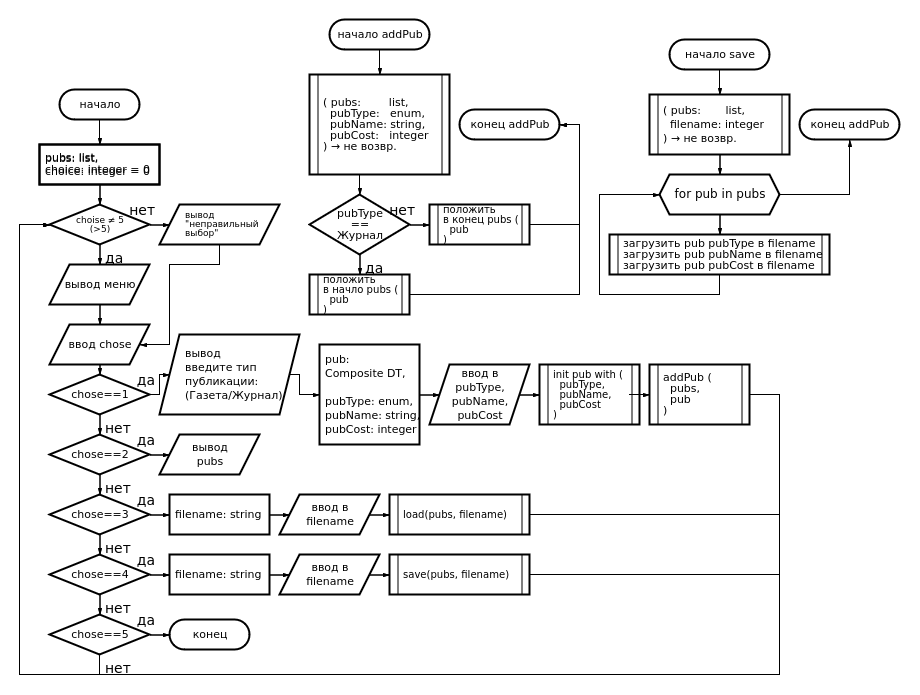
\includegraphics[width=0.8\textwidth]{data/diagram16_2.png}
\end{figure}
\subsection{Код:}
\verbatiminput{data/task16_2.cpp}
\href{https://raw.githubusercontent.com/John1400800/stuff/refs/heads/main/c_learning/home_works/task16_2.cpp}{source code}
\newpage
\subsection{Результат работы программы}
\begin{figure}[h]
    % \centering
    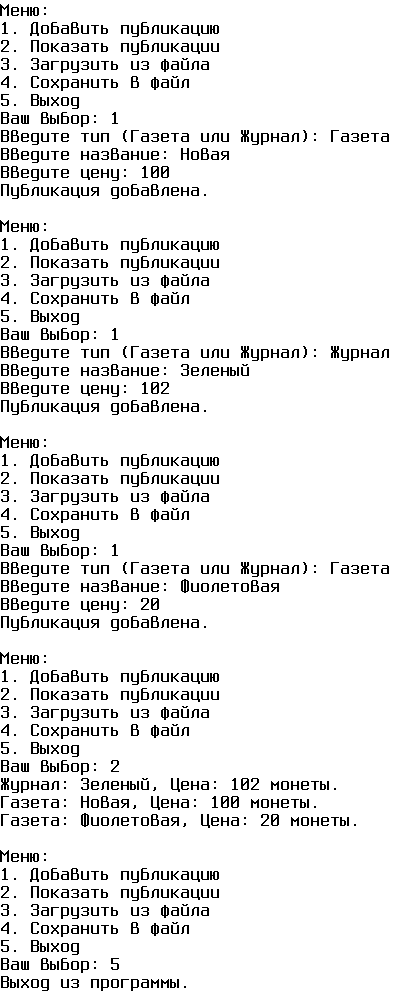
\includegraphics[height=0.5\textheight]{data/demo16_2.png}
\end{figure}

\section*{Задание 3}

\setcounter{subsection}{0} % подпункты с 1

\subsection{Условие:}
\begin{figure}[h]
    \centering
    
\includegraphics[width=0.8\textwidth]{data/condition16_3.png}
\end{figure}

\subsection{Алгоритм / Математическая модель}

Программа предназначена для работы с многочленами (полиномами) и позволяет добавлять, удалять и отображать члены полинома. Алгоритм выполнения программы следующий:

\begin{enumerate}
\item \textbf{Меню:} программа предлагает пользователю выбор действий через консоль:
\begin{itemize}
\item Ввести новый член полинома.
\item Удалить член полинома по указанной степени.
\item Вывести полином на экран.
\item Выйти из программы.
\end{itemize}

\item \textbf{Ввести новый член полинома:}
\begin{itemize}
\item Запрашивает у пользователя многочлен или одночлен в строковом формате.
\item Строка анализируется на наличие коэффициента и степени переменной.
\item Если степень не указана, то по умолчанию считается, что степень равна 1.
\item Добавляет новый член полинома в список. Если степень уже существует, коэффициенты складываются.
\end{itemize}

\item \textbf{Удалить член полинома по указанной степени:}
\begin{itemize}
\item Программа запрашивает у пользователя степень члена, который нужно удалить.
\item Если в полиноме существует член с указанной степенью, он удаляется из списка.
\end{itemize}

\item \textbf{Вывести полином:}
\begin{itemize}
\item Программа выводит все члены полинома в формате: коэффициент, переменная, степень.
\item Если полином пуст, выводится сообщение "Полином пуст".
\end{itemize}

\item \textbf{Выход:} программа завершает свою работу.

\end{enumerate}
{\large\textbf{\\[2mm]2.1 Математическая модель}}

\begin{enumerate}
\item \textbf{Член полинома} (терм) представляется как пара:
\[
T(x) = (a, n)
\]
где \(a\) — коэффициент, а \(n\) — степень переменной \(x\).

\item \textbf{Полином} состоит из списка членов, каждый из которых представляет собой пару \((a, n)\), где \(a\) — коэффициент, а \(n\) — степень.

\item \textbf{Процесс парсинга строки}:
    - Если строка содержит символ 'x', то извлекаются коэффициент и степень.
    - Если 'x' отсутствует, то это константа (степень 0, коэффициент равен числу).
    - Если степень не указана явно, то она считается равной 1.

\item \textbf{Алгоритм добавления члена в полином}:
    - Если степень уже присутствует в полиноме, то коэффициенты складываются.
    - Если степень отсутствует, новый член вставляется в нужное место, поддерживая упорядоченность полинома по убыванию степени.

\item \textbf{Удаление члена по степени}:
    - Процесс удаления члена полинома с указанной степенью из списка.

\item \textbf{Вывод полинома}:
    - Все члены полинома выводятся в читаемом виде, с учетом знака коэффициента, степени и форматирования.

Таким образом, программа позволяет эффективно манипулировать многочленами, обеспечивая функции для их редактирования и отображения.
\end{enumerate}
\subsection{Диаграмма:}
\begin{figure}[h]
    \centering
    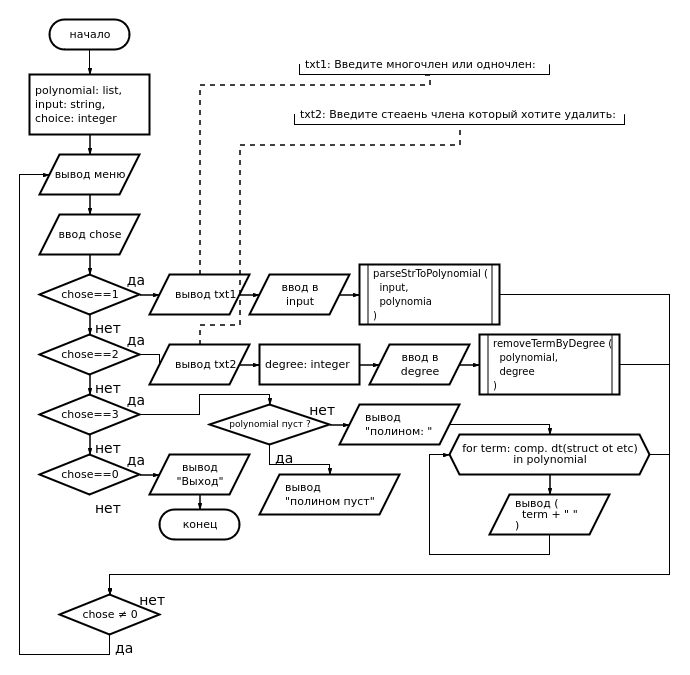
\includegraphics[width=0.8\textwidth]{data/diagram16_3.png}
\end{figure}
\subsection{Код:}
\verbatiminput{data/task16_3.cpp}
\href{https://raw.githubusercontent.com/John1400800/stuff/refs/heads/main/c_learning/home_works/task16_3.cpp}{source code}
\newpage
\subsection{Результат работы программы}
\begin{figure}[h]
    % \centering
    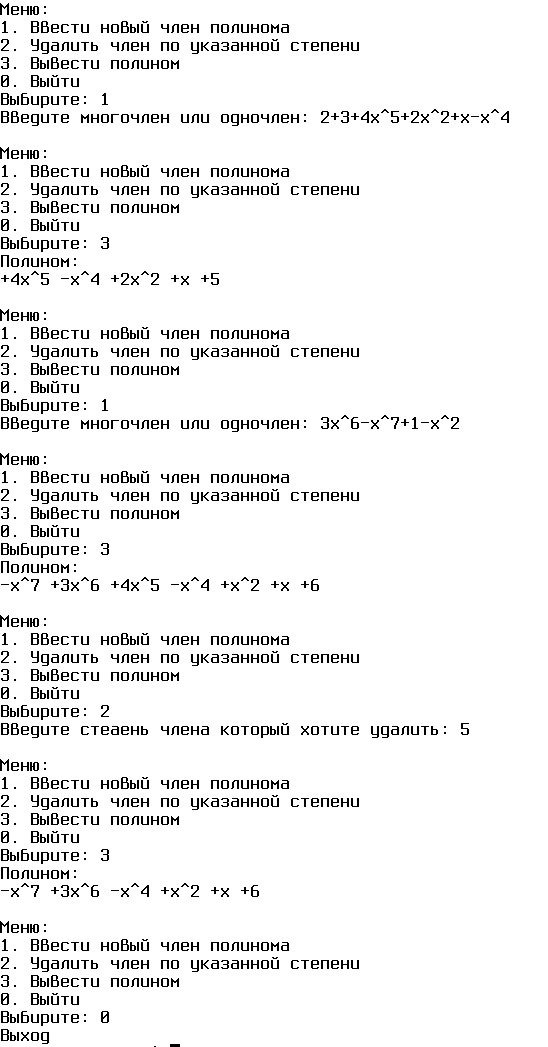
\includegraphics[height=0.5\textheight]{data/demo16_3.png}
\end{figure}
\end{document}
